%%%%%%%%%%%%%%%%%%%%%%%%%%%%%%%%%%%%%%%%%%%%%%%%%%
% Part: Introduction
% Filename: intro.tex
% Created: September 9, 2017
% Author: Adam Wright
%%%%%%%%%%%%%%%%%%%%%%%%%%%%%%%%%%%%%%%%%%%%%%%%%%



%%%%%%%%%%%%%%%%%%%%%%%%%%%%%%%%%%%%%%%%%%%%%%%%%%
% Introduction
%%%%%%%%%%%%%%%%%%%%%%%%%%%%%%%%%%%%%%%%%%%%%%%%%%
\chapter{Introduction}
In 1609, Galileo Galilei aimed a device of two lenses at the sky, seeing for the first time with magnification the imperfections on the moon, small objects orbiting Jupiter, and even the phases of Venus (Keck Observatory, ``A history of telescopes''). With observations from this crude contraption, Galileo revolutionized what was believed of the solar system by showing the Sun, not the Earth, was at the center of the solar system. As time progressed, inquisitive minds began to wonder what else could be discovered with the power of magnification. Telescopes, as they were soon coined, began to be advanced heavily. Lenses were made larger in diameter in order to view fainter objects. Optical components were fabricated with less imperfection allowing for better resolution. Curvature and focal lengths of lenses were exploited, allowing for varying degrees of magnification. Achromatic, aspheric, and cylindrical lenses were created, ridding telescopes of many aberrations. By the late twentieth century, telescopes were as optically perfect as they could be; no advancements in optics would allow them to see with greater magnification or increased resolution. However, there was one lingering problem.

Light can be approximated as a ray. This means that as it travels through free space, it travels in a straight line and does not deviate from the path. Suppose, however, that this ray of light travels from free space into a region of gas. Will the ray continue to travel in a straight line as it passes through the gas? The solution to this problem is the famous Snell's Law, given in Equation \ref{snellslaw}, which tells us that it will not continue in a straight line, but will bend, or \textit{refract}. As shown in Figure \ref{snellsfigure}, consider a ray of light travelling through free space of index of refraction $n_1$. As it comes into contact with the gas, denote the angle it makes to the normal of the boundary between the gas and free space by $\theta_1$. As it passes into the gas of index of refraction $n_2$, denote the angle it makes with the normal on the opposite side of the boundary as $\theta_2$. Snell's Law tells us how to relate these quantities:

\begin{equation}
  n_1 \sin \theta_1 = n_2 \sin \theta_2
  \label{snellslaw}
\end{equation}



\begin{figure}
  \center
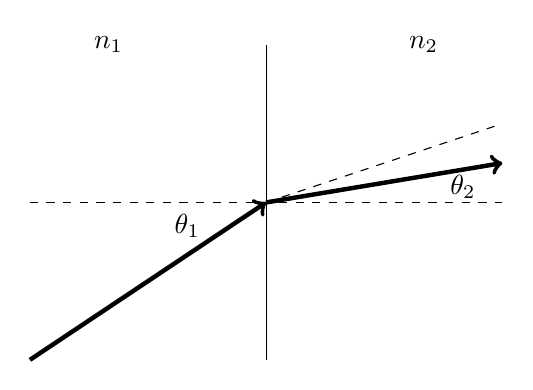
\begin{tikzpicture}
  \node(n1) at (0,0) {$n_1$};
  \node[right of = n1,node distance = 4cm](n2) {$n_2$};
  \draw (2,0) -- (2,-4);
  \draw[->, line width = 1.6pt] (-1,-4) -- (2,-2); 
  \draw[dashed] (2,-2) -- (5,-1); 
  \draw[dashed] (-1,-2) -- (5,-2); 
  \draw[->,line width = 1.6pt] (2,-2) -- (5,-1.5);
  \node(thetaone) at (1,-2.3) {$\theta_1$};
  \node(thetatwo) at (4.5,-1.8) {$\theta_2$};
\end{tikzpicture}
\caption{A figure of Snell's Law}
\label{snellsfigure}
\end{figure}
Returning to the idea of telescopes, light that is emitted from a distant star or reflected off a moon or planet will essentially travel through free space for the majority of its voyage. However, as it nears Earth, it begins to enter the atmosphere that surrounds Earth, and refracts according to Snell's Law. It would seem that this refraction is the same for all rays of light, and thus does not result in any imperfections when imaging with a telescope. The problem stems from two issues: The first issue is that the index of refraction depends on many parameters such as temperature, pressure, and density. The second issue is that the atmosphere of the Earth is not constant in these parameters, but fluctuates slightly over time. Putting this two issues together tells us that light will not refract uniformly as it passes through the atmosphere, but will be distorted due to fluctuations in the index of refraction. This is known as atmospheric distortion.


In order for telescopes to receive clearer images, astronomers would need to find a way to rid their systems of atmospheric distortion. One way to do this would be to put a telescope outside of Earth's atmosphere; this was done with amazing success (apart from an initial hiccup) in 1990 with the Hubble Telescope, a low orbiting, powerful telescope. However, it is not only extremely costly to put telescopes into orbit, but also difficult as they cannot be easily maintained or services.

Thus, a different solution was posed. If the astronomers could somehow model how light was distorted as it entered the atmosphere, they could then subtract those distortions out of their images and obtain clearer data? The answer was yes. By observing a point source in the sky, such as a distant star, and knowing how a point source would ideally be imaged through their telescope, they could compare the distorted image of the point source with what the point source would ideally look like and correct their data.

This process became known as adaptive optics and is used by many ground-based telescopes around the world. Telescopes observe a distant star, or a man-made ``laser guide star,'' compare it to an ideally images point source, and move a deformable mirror to subtract out distortions. The result is crystal clear images without atmospheric distortion.

